\documentclass[1p]{elsarticle_modified}
%\bibliographystyle{elsarticle-num}

%\usepackage[colorlinks]{hyperref}
%\usepackage{abbrmath_seonhwa} %\Abb, \Ascr, \Acal ,\Abf, \Afrak
\usepackage{amsfonts}
\usepackage{amssymb}
\usepackage{amsmath}
\usepackage{amsthm}
\usepackage{scalefnt}
\usepackage{amsbsy}
\usepackage{kotex}
\usepackage{caption}
\usepackage{subfig}
\usepackage{color}
\usepackage{graphicx}
\usepackage{xcolor} %% white, black, red, green, blue, cyan, magenta, yellow
\usepackage{float}
\usepackage{setspace}
\usepackage{hyperref}

\usepackage{tikz}
\usetikzlibrary{arrows}

\usepackage{multirow}
\usepackage{array} % fixed length table
\usepackage{hhline}

%%%%%%%%%%%%%%%%%%%%%
\makeatletter
\renewcommand*\env@matrix[1][\arraystretch]{%
	\edef\arraystretch{#1}%
	\hskip -\arraycolsep
	\let\@ifnextchar\new@ifnextchar
	\array{*\c@MaxMatrixCols c}}
\makeatother %https://tex.stackexchange.com/questions/14071/how-can-i-increase-the-line-spacing-in-a-matrix
%%%%%%%%%%%%%%%

\usepackage[normalem]{ulem}

\newcommand{\msout}[1]{\ifmmode\text{\sout{\ensuremath{#1}}}\else\sout{#1}\fi}
%SOURCE: \msout is \stkout macro in https://tex.stackexchange.com/questions/20609/strikeout-in-math-mode

\newcommand{\cancel}[1]{
	\ifmmode
	{\color{red}\msout{#1}}
	\else
	{\color{red}\sout{#1}}
	\fi
}

\newcommand{\add}[1]{
	{\color{blue}\uwave{#1}}
}

\newcommand{\replace}[2]{
	\ifmmode
	{\color{red}\msout{#1}}{\color{blue}\uwave{#2}}
	\else
	{\color{red}\sout{#1}}{\color{blue}\uwave{#2}}
	\fi
}

\newcommand{\Sol}{\mathcal{S}} %segment
\newcommand{\D}{D} %diagram
\newcommand{\A}{\mathcal{A}} %arc


%%%%%%%%%%%%%%%%%%%%%%%%%%%%%5 test

\def\sl{\operatorname{\textup{SL}}(2,\Cbb)}
\def\psl{\operatorname{\textup{PSL}}(2,\Cbb)}
\def\quan{\mkern 1mu \triangleright \mkern 1mu}

\theoremstyle{definition}
\newtheorem{thm}{Theorem}[section]
\newtheorem{prop}[thm]{Proposition}
\newtheorem{lem}[thm]{Lemma}
\newtheorem{ques}[thm]{Question}
\newtheorem{cor}[thm]{Corollary}
\newtheorem{defn}[thm]{Definition}
\newtheorem{exam}[thm]{Example}
\newtheorem{rmk}[thm]{Remark}
\newtheorem{alg}[thm]{Algorithm}

\newcommand{\I}{\sqrt{-1}}
\begin{document}

%\begin{frontmatter}
%
%\title{Boundary parabolic representations of knots up to 8 crossings}
%
%%% Group authors per affiliation:
%\author{Yunhi Cho} 
%\address{Department of Mathematics, University of Seoul, Seoul, Korea}
%\ead{yhcho@uos.ac.kr}
%
%
%\author{Seonhwa Kim} %\fnref{s_kim}}
%\address{Center for Geometry and Physics, Institute for Basic Science, Pohang, 37673, Korea}
%\ead{ryeona17@ibs.re.kr}
%
%\author{Hyuk Kim}
%\address{Department of Mathematical Sciences, Seoul National University, Seoul 08826, Korea}
%\ead{hyukkim@snu.ac.kr}
%
%\author{Seokbeom Yoon}
%\address{Department of Mathematical Sciences, Seoul National University, Seoul, 08826,  Korea}
%\ead{sbyoon15@snu.ac.kr}
%
%\begin{abstract}
%We find all boundary parabolic representation of knots up to 8 crossings.
%
%\end{abstract}
%\begin{keyword}
%    \MSC[2010] 57M25 
%\end{keyword}
%
%\end{frontmatter}

%\linenumbers
%\tableofcontents
%
\newcommand\colored[1]{\textcolor{white}{\rule[-0.35ex]{0.8em}{1.4ex}}\kern-0.8em\color{red} #1}%
%\newcommand\colored[1]{\textcolor{white}{ #1}\kern-2.17ex	\textcolor{white}{ #1}\kern-1.81ex	\textcolor{white}{ #1}\kern-2.15ex\color{red}#1	}

{\Large $\underline{12a_{1221}~(K12a_{1221})}$}

\setlength{\tabcolsep}{10pt}
\renewcommand{\arraystretch}{1.6}
\vspace{1cm}\begin{tabular}{m{100pt}>{\centering\arraybackslash}m{274pt}}
\multirow{5}{120pt}{
	\centering
	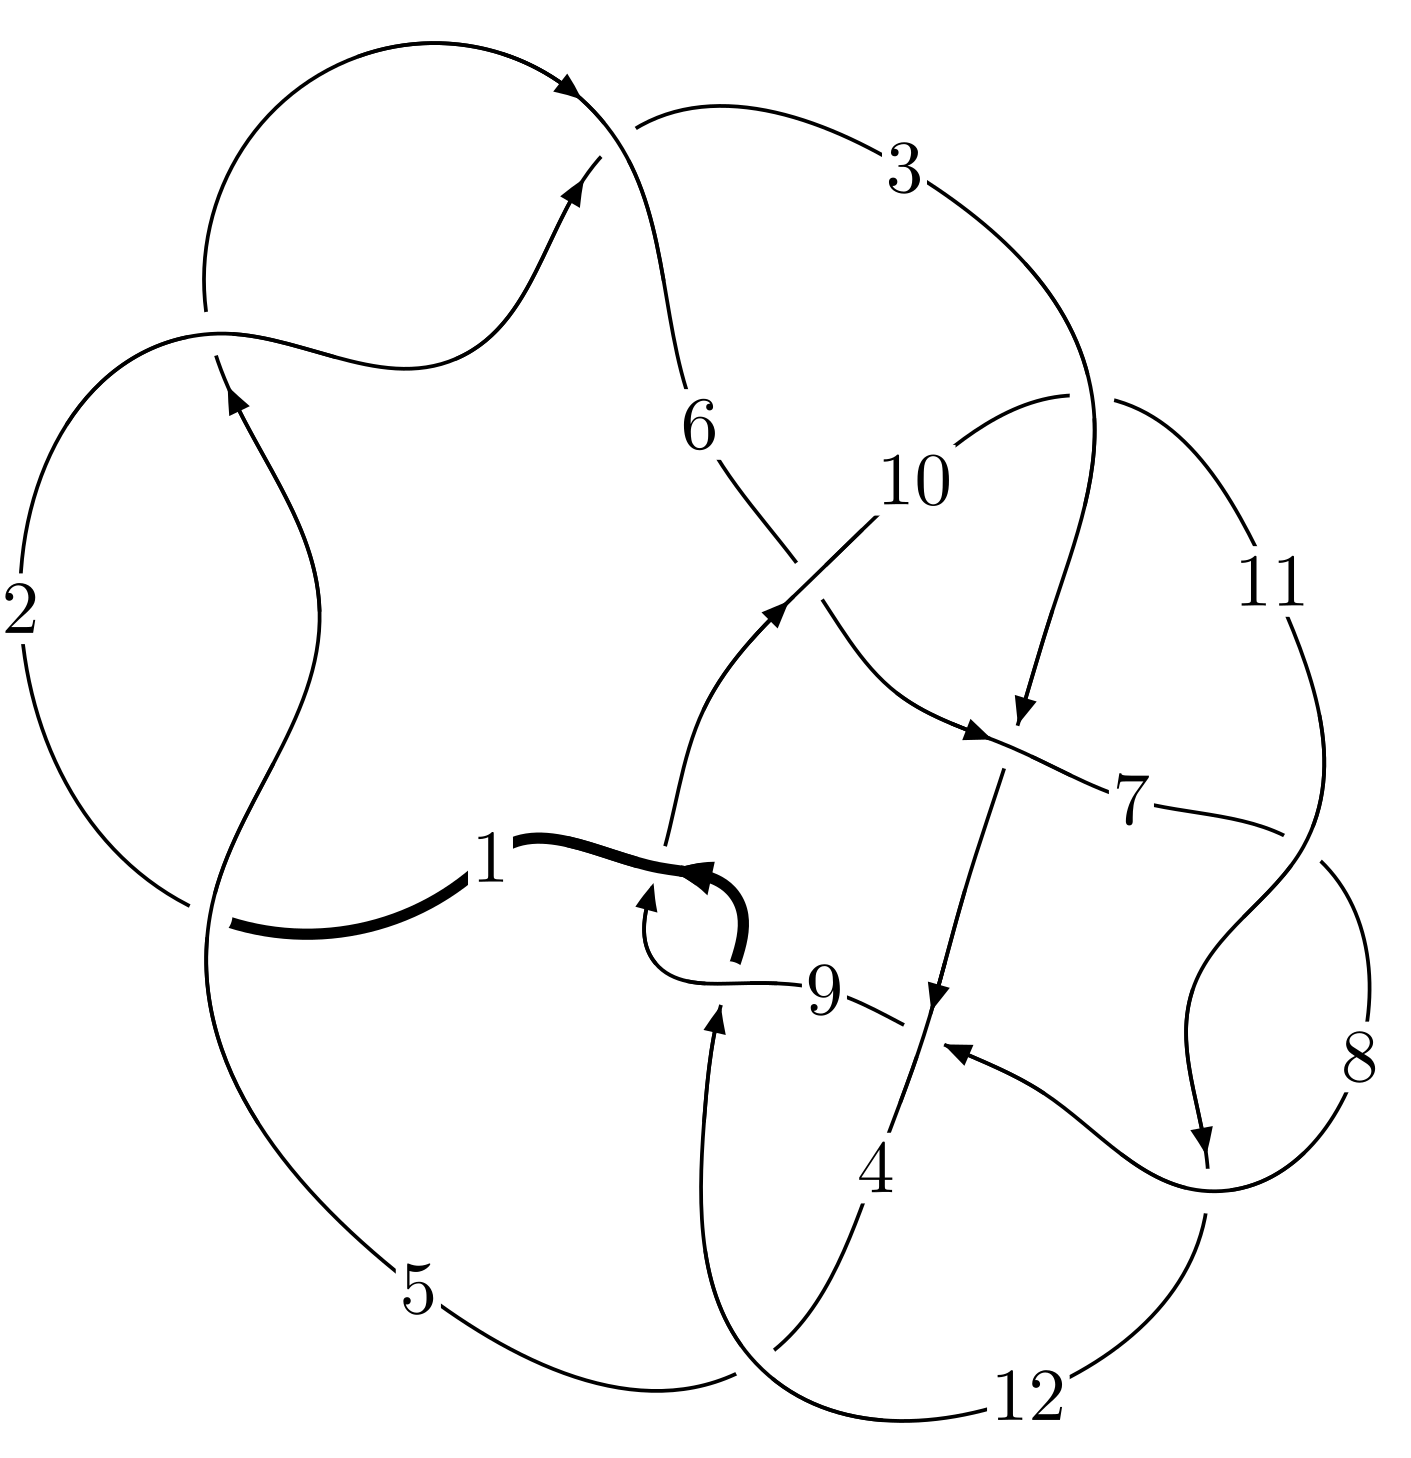
\includegraphics[width=112pt]{../../../GIT/diagram.site/Diagrams/png/2022_12a_1221.png}\\
\ \ \ A knot diagram\footnotemark}&
\allowdisplaybreaks
\textbf{Linearized knot diagam} \\
\cline{2-2}
 &
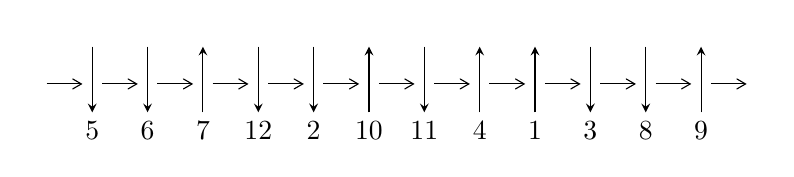
\begin{tikzpicture}[x=20pt, y=17pt]
	% nodes
	\node (C0) at (0, 0) {};
	\node (C1) at (1, 0) {};
	\node (C1U) at (1, +1) {};
	\node (C1D) at (1, -1) {5};

	\node (C2) at (2, 0) {};
	\node (C2U) at (2, +1) {};
	\node (C2D) at (2, -1) {6};

	\node (C3) at (3, 0) {};
	\node (C3U) at (3, +1) {};
	\node (C3D) at (3, -1) {7};

	\node (C4) at (4, 0) {};
	\node (C4U) at (4, +1) {};
	\node (C4D) at (4, -1) {12};

	\node (C5) at (5, 0) {};
	\node (C5U) at (5, +1) {};
	\node (C5D) at (5, -1) {2};

	\node (C6) at (6, 0) {};
	\node (C6U) at (6, +1) {};
	\node (C6D) at (6, -1) {10};

	\node (C7) at (7, 0) {};
	\node (C7U) at (7, +1) {};
	\node (C7D) at (7, -1) {11};

	\node (C8) at (8, 0) {};
	\node (C8U) at (8, +1) {};
	\node (C8D) at (8, -1) {4};

	\node (C9) at (9, 0) {};
	\node (C9U) at (9, +1) {};
	\node (C9D) at (9, -1) {1};

	\node (C10) at (10, 0) {};
	\node (C10U) at (10, +1) {};
	\node (C10D) at (10, -1) {3};

	\node (C11) at (11, 0) {};
	\node (C11U) at (11, +1) {};
	\node (C11D) at (11, -1) {8};

	\node (C12) at (12, 0) {};
	\node (C12U) at (12, +1) {};
	\node (C12D) at (12, -1) {9};
	\node (C13) at (13, 0) {};

	% arrows
	\draw[->,>={angle 60}]
	(C0) edge (C1) (C1) edge (C2) (C2) edge (C3) (C3) edge (C4) (C4) edge (C5) (C5) edge (C6) (C6) edge (C7) (C7) edge (C8) (C8) edge (C9) (C9) edge (C10) (C10) edge (C11) (C11) edge (C12) (C12) edge (C13) ;	\draw[->,>=stealth]
	(C1U) edge (C1D) (C2U) edge (C2D) (C3D) edge (C3U) (C4U) edge (C4D) (C5U) edge (C5D) (C6D) edge (C6U) (C7U) edge (C7D) (C8D) edge (C8U) (C9D) edge (C9U) (C10U) edge (C10D) (C11U) edge (C11D) (C12D) edge (C12U) ;
	\end{tikzpicture} \\
\hhline{~~} \\& 
\textbf{Solving Sequence} \\ \cline{2-2} 
 &
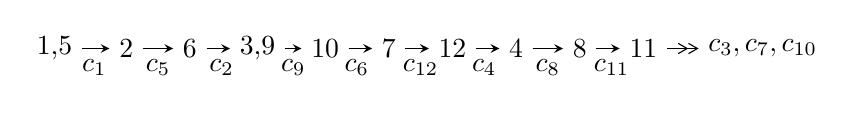
\begin{tikzpicture}[x=23pt, y=7pt]
	% node
	\node (A0) at (-1/8, 0) {1,5};
	\node (A1) at (1, 0) {2};
	\node (A2) at (2, 0) {6};
	\node (A3) at (49/16, 0) {3,9};
	\node (A4) at (33/8, 0) {10};
	\node (A5) at (41/8, 0) {7};
	\node (A6) at (49/8, 0) {12};
	\node (A7) at (57/8, 0) {4};
	\node (A8) at (65/8, 0) {8};
	\node (A9) at (73/8, 0) {11};
	\node (C1) at (1/2, -1) {$c_{1}$};
	\node (C2) at (3/2, -1) {$c_{5}$};
	\node (C3) at (5/2, -1) {$c_{2}$};
	\node (C4) at (29/8, -1) {$c_{9}$};
	\node (C5) at (37/8, -1) {$c_{6}$};
	\node (C6) at (45/8, -1) {$c_{12}$};
	\node (C7) at (53/8, -1) {$c_{4}$};
	\node (C8) at (61/8, -1) {$c_{8}$};
	\node (C9) at (69/8, -1) {$c_{11}$};
	\node (A10) at (11, 0) {$c_{3},c_{7},c_{10}$};

	% edge
	\draw[->,>=stealth]	
	(A0) edge (A1) (A1) edge (A2) (A2) edge (A3) (A3) edge (A4) (A4) edge (A5) (A5) edge (A6) (A6) edge (A7) (A7) edge (A8) (A8) edge (A9) ;
	\draw[->>,>={angle 60}]	
	(A9) edge (A10);
\end{tikzpicture} \\ 

\end{tabular} \\

\footnotetext{
The image of knot diagram is generated by the software ``\textbf{Draw programme}" developed by Andrew Bartholomew(\url{http://www.layer8.co.uk/maths/draw/index.htm\#Running-draw}), where we modified some parts for our purpose(\url{https://github.com/CATsTAILs/LinksPainter}).
}\phantom \\ \newline 
\centering \textbf{Ideals for irreducible components\footnotemark of $X_{\text{par}}$} 
 
\begin{align*}
I^u_{1}&=\langle 
6.28820\times10^{367} u^{121}-1.15899\times10^{368} u^{120}+\cdots+2.80418\times10^{367} b+5.57387\times10^{368},\\
\phantom{I^u_{1}}&\phantom{= \langle  }6.96628\times10^{366} u^{121}-2.09868\times10^{367} u^{120}+\cdots+1.12167\times10^{367} a+4.96920\times10^{368},\\
\phantom{I^u_{1}}&\phantom{= \langle  }u^{122}-2 u^{121}+\cdots+47 u+1\rangle \\
I^u_{2}&=\langle 
-182 u^{19}-1044 u^{18}+\cdots+101 b+381,\;2772 u^{19}+7347 u^{18}+\cdots+101 a-2400,\\
\phantom{I^u_{2}}&\phantom{= \langle  }u^{20}+4 u^{19}+\cdots-5 u-1\rangle \\
I^u_{3}&=\langle 
b,\;a+1,\;u-1\rangle \\
I^u_{4}&=\langle 
b+a-1,\;a^2-2 a-1,\;u-1\rangle \\
I^u_{5}&=\langle 
b+2 a+2,\;2 a^2+4 a+1,\;u-1\rangle \\
\\
\end{align*}
\raggedright * 5 irreducible components of $\dim_{\mathbb{C}}=0$, with total 147 representations.\\
\footnotetext{All coefficients of polynomials are rational numbers. But the coefficients are sometimes approximated in decimal forms when there is not enough margin.}
\newpage
\renewcommand{\arraystretch}{1}
\centering \section*{I. $I^u_{1}= \langle 6.29\times10^{367} u^{121}-1.16\times10^{368} u^{120}+\cdots+2.80\times10^{367} b+5.57\times10^{368},\;6.97\times10^{366} u^{121}-2.10\times10^{367} u^{120}+\cdots+1.12\times10^{367} a+4.97\times10^{368},\;u^{122}-2 u^{121}+\cdots+47 u+1 \rangle$}
\flushleft \textbf{(i) Arc colorings}\\
\begin{tabular}{m{7pt} m{180pt} m{7pt} m{180pt} }
\flushright $a_{1}=$&$\begin{pmatrix}1\\0\end{pmatrix}$ \\
\flushright $a_{5}=$&$\begin{pmatrix}0\\u\end{pmatrix}$ \\
\flushright $a_{2}=$&$\begin{pmatrix}1\\u^2\end{pmatrix}$ \\
\flushright $a_{6}=$&$\begin{pmatrix}- u\\- u^3+u\end{pmatrix}$ \\
\flushright $a_{3}=$&$\begin{pmatrix}- u^2+1\\- u^4+2 u^2\end{pmatrix}$ \\
\flushright $a_{9}=$&$\begin{pmatrix}-0.621063 u^{121}+1.87103 u^{120}+\cdots-319.578 u-44.3017\\-2.24244 u^{121}+4.13307 u^{120}+\cdots-767.054 u-19.8770\end{pmatrix}$ \\
\flushright $a_{10}=$&$\begin{pmatrix}-2.86350 u^{121}+6.00410 u^{120}+\cdots-1086.63 u-64.1787\\-2.24244 u^{121}+4.13307 u^{120}+\cdots-767.054 u-19.8770\end{pmatrix}$ \\
\flushright $a_{7}=$&$\begin{pmatrix}-15.5463 u^{121}+33.3435 u^{120}+\cdots-5050.45 u-174.308\\1.98458 u^{121}-4.93885 u^{120}+\cdots+87.1412 u-1.41589\end{pmatrix}$ \\
\flushright $a_{12}=$&$\begin{pmatrix}4.21410 u^{121}-8.25746 u^{120}+\cdots+3320.96 u+137.229\\-1.32201 u^{121}+3.30816 u^{120}+\cdots+170.879 u+7.81217\end{pmatrix}$ \\
\flushright $a_{4}=$&$\begin{pmatrix}-17.4596 u^{121}+36.3324 u^{120}+\cdots-6283.25 u-247.315\\-2.24708 u^{121}+5.66160 u^{120}+\cdots-469.534 u-15.1655\end{pmatrix}$ \\
\flushright $a_{8}=$&$\begin{pmatrix}14.2213 u^{121}-30.2530 u^{120}+\cdots+5516.59 u+223.332\\-1.91058 u^{121}+4.28655 u^{120}+\cdots-464.676 u-7.01531\end{pmatrix}$ \\
\flushright $a_{11}=$&$\begin{pmatrix}-1.13844 u^{121}+3.06041 u^{120}+\cdots-402.877 u-46.3036\\-2.28437 u^{121}+4.20143 u^{120}+\cdots-762.095 u-19.6846\end{pmatrix}$\\&\end{tabular}
\flushleft \textbf{(ii) Obstruction class $= -1$}\\~\\
\flushleft \textbf{(iii) Cusp Shapes $= -19.4694 u^{121}+41.3664 u^{120}+\cdots-2930.19 u-56.4322$}\\~\\
\newpage\renewcommand{\arraystretch}{1}
\flushleft \textbf{(iv) u-Polynomials at the component}\newline \\
\begin{tabular}{m{50pt}|m{274pt}}
Crossings & \hspace{64pt}u-Polynomials at each crossing \\
\hline $$\begin{aligned}c_{1},c_{2},c_{5}\end{aligned}$$&$\begin{aligned}
&u^{122}+2 u^{121}+\cdots-47 u+1
\end{aligned}$\\
\hline $$\begin{aligned}c_{3}\end{aligned}$$&$\begin{aligned}
&u^{122}+6 u^{121}+\cdots+56 u-226
\end{aligned}$\\
\hline $$\begin{aligned}c_{4}\end{aligned}$$&$\begin{aligned}
&u^{122}- u^{121}+\cdots-4608 u+1408
\end{aligned}$\\
\hline $$\begin{aligned}c_{6}\end{aligned}$$&$\begin{aligned}
&u^{122}-5 u^{121}+\cdots+33792 u+4096
\end{aligned}$\\
\hline $$\begin{aligned}c_{7},c_{11}\end{aligned}$$&$\begin{aligned}
&u^{122}+u^{121}+\cdots-266 u-7
\end{aligned}$\\
\hline $$\begin{aligned}c_{8}\end{aligned}$$&$\begin{aligned}
&2(2 u^{122}-15 u^{120}+\cdots-130 u+4)
\end{aligned}$\\
\hline $$\begin{aligned}c_{9},c_{12}\end{aligned}$$&$\begin{aligned}
&u^{122}-39 u^{120}+\cdots+24316 u-3428
\end{aligned}$\\
\hline $$\begin{aligned}c_{10}\end{aligned}$$&$\begin{aligned}
&2(2 u^{122}-6 u^{121}+\cdots+323446 u-14731)
\end{aligned}$\\
\hline
\end{tabular}\\~\\
\newpage\renewcommand{\arraystretch}{1}
\flushleft \textbf{(v) Riley Polynomials at the component}\newline \\
\begin{tabular}{m{50pt}|m{274pt}}
Crossings & \hspace{64pt}Riley Polynomials at each crossing \\
\hline $$\begin{aligned}c_{1},c_{2},c_{5}\end{aligned}$$&$\begin{aligned}
&y^{122}-130 y^{121}+\cdots-679 y+1
\end{aligned}$\\
\hline $$\begin{aligned}c_{3}\end{aligned}$$&$\begin{aligned}
&y^{122}-8 y^{121}+\cdots+969116 y+51076
\end{aligned}$\\
\hline $$\begin{aligned}c_{4}\end{aligned}$$&$\begin{aligned}
&y^{122}-29 y^{121}+\cdots-133603328 y+1982464
\end{aligned}$\\
\hline $$\begin{aligned}c_{6}\end{aligned}$$&$\begin{aligned}
&y^{122}+9 y^{121}+\cdots+167247872 y+16777216
\end{aligned}$\\
\hline $$\begin{aligned}c_{7},c_{11}\end{aligned}$$&$\begin{aligned}
&y^{122}-93 y^{121}+\cdots-12124 y+49
\end{aligned}$\\
\hline $$\begin{aligned}c_{8}\end{aligned}$$&$\begin{aligned}
&4(4 y^{122}-60 y^{121}+\cdots-9596 y+16)
\end{aligned}$\\
\hline $$\begin{aligned}c_{9},c_{12}\end{aligned}$$&$\begin{aligned}
&y^{122}-78 y^{121}+\cdots-551516768 y+11751184
\end{aligned}$\\
\hline $$\begin{aligned}c_{10}\end{aligned}$$&$\begin{aligned}
&4(4 y^{122}-192 y^{121}+\cdots-4.02466\times10^{10} y+2.17002\times10^{8})
\end{aligned}$\\
\hline
\end{tabular}\\~\\
\newpage\flushleft \textbf{(vi) Complex Volumes and Cusp Shapes}
$$\begin{array}{c|c|c}  
\text{Solutions to }I^u_{1}& \I (\text{vol} + \sqrt{-1}CS) & \text{Cusp shape}\\
 \hline 
\begin{aligned}
u &= \phantom{-}0.775615 + 0.632204 I \\
a &= -0.012407 - 0.325555 I \\
b &= \phantom{-}0.177801 + 0.559881 I\end{aligned}
 & -4.90234 - 0.58995 I & \phantom{-0.000000 } 0 \\ \hline\begin{aligned}
u &= \phantom{-}0.775615 - 0.632204 I \\
a &= -0.012407 + 0.325555 I \\
b &= \phantom{-}0.177801 - 0.559881 I\end{aligned}
 & -4.90234 + 0.58995 I & \phantom{-0.000000 } 0 \\ \hline\begin{aligned}
u &= \phantom{-}0.866013 + 0.476254 I \\
a &= \phantom{-}1.79771 + 0.27061 I \\
b &= -1.341600 + 0.061557 I\end{aligned}
 & -0.249126 + 0.781997 I & \phantom{-0.000000 } 0 \\ \hline\begin{aligned}
u &= \phantom{-}0.866013 - 0.476254 I \\
a &= \phantom{-}1.79771 - 0.27061 I \\
b &= -1.341600 - 0.061557 I\end{aligned}
 & -0.249126 - 0.781997 I & \phantom{-0.000000 } 0 \\ \hline\begin{aligned}
u &= \phantom{-}0.409705 + 0.898488 I \\
a &= -2.12084 - 0.15136 I \\
b &= \phantom{-}1.138670 - 0.362404 I\end{aligned}
 & -2.10139 - 4.17725 I & \phantom{-0.000000 } 0 \\ \hline\begin{aligned}
u &= \phantom{-}0.409705 - 0.898488 I \\
a &= -2.12084 + 0.15136 I \\
b &= \phantom{-}1.138670 + 0.362404 I\end{aligned}
 & -2.10139 + 4.17725 I & \phantom{-0.000000 } 0 \\ \hline\begin{aligned}
u &= \phantom{-}0.377143 + 0.909077 I \\
a &= \phantom{-}1.70164 + 0.27529 I \\
b &= -1.031380 + 0.284248 I\end{aligned}
 & \phantom{-}0.99667 - 3.65957 I & \phantom{-0.000000 } 0 \\ \hline\begin{aligned}
u &= \phantom{-}0.377143 - 0.909077 I \\
a &= \phantom{-}1.70164 - 0.27529 I \\
b &= -1.031380 - 0.284248 I\end{aligned}
 & \phantom{-}0.99667 + 3.65957 I & \phantom{-0.000000 } 0 \\ \hline\begin{aligned}
u &= -0.576185 + 0.775295 I \\
a &= \phantom{-}1.65486 - 0.51228 I \\
b &= -1.313900 - 0.454283 I\end{aligned}
 & \phantom{-}4.67316 + 8.47858 I & \phantom{-0.000000 } 0 \\ \hline\begin{aligned}
u &= -0.576185 - 0.775295 I \\
a &= \phantom{-}1.65486 + 0.51228 I \\
b &= -1.313900 + 0.454283 I\end{aligned}
 & \phantom{-}4.67316 - 8.47858 I & \phantom{-0.000000 } 0\\
 \hline 
 \end{array}$$\newpage$$\begin{array}{c|c|c}  
\text{Solutions to }I^u_{1}& \I (\text{vol} + \sqrt{-1}CS) & \text{Cusp shape}\\
 \hline 
\begin{aligned}
u &= \phantom{-}0.352255 + 0.979492 I \\
a &= -1.197070 - 0.034278 I \\
b &= \phantom{-}0.697958 - 0.393964 I\end{aligned}
 & -3.30086 - 4.68037 I & \phantom{-0.000000 } 0 \\ \hline\begin{aligned}
u &= \phantom{-}0.352255 - 0.979492 I \\
a &= -1.197070 + 0.034278 I \\
b &= \phantom{-}0.697958 + 0.393964 I\end{aligned}
 & -3.30086 + 4.68037 I & \phantom{-0.000000 } 0 \\ \hline\begin{aligned}
u &= -0.522215 + 0.801277 I \\
a &= \phantom{-}1.23040 - 0.76678 I \\
b &= -1.184080 + 0.229121 I\end{aligned}
 & \phantom{-}4.85947 - 3.25008 I & \phantom{-0.000000 } 0 \\ \hline\begin{aligned}
u &= -0.522215 - 0.801277 I \\
a &= \phantom{-}1.23040 + 0.76678 I \\
b &= -1.184080 - 0.229121 I\end{aligned}
 & \phantom{-}4.85947 + 3.25008 I & \phantom{-0.000000 } 0 \\ \hline\begin{aligned}
u &= \phantom{-}1.07777\phantom{ +0.000000I} \\
a &= -0.141435\phantom{ +0.000000I} \\
b &= \phantom{-}1.49397\phantom{ +0.000000I}\end{aligned}
 & \phantom{-}3.19101\phantom{ +0.000000I} & \phantom{-0.000000 } 0 \\ \hline\begin{aligned}
u &= \phantom{-}1.10589\phantom{ +0.000000I} \\
a &= -2.28955\phantom{ +0.000000I} \\
b &= \phantom{-}1.39337\phantom{ +0.000000I}\end{aligned}
 & \phantom{-}2.70025\phantom{ +0.000000I} & \phantom{-0.000000 } 0 \\ \hline\begin{aligned}
u &= -0.602865 + 0.935266 I \\
a &= -1.71285 + 0.28050 I \\
b &= \phantom{-}1.299420 + 0.481580 I\end{aligned}
 & -0.62473 + 13.83740 I & \phantom{-0.000000 } 0 \\ \hline\begin{aligned}
u &= -0.602865 - 0.935266 I \\
a &= -1.71285 - 0.28050 I \\
b &= \phantom{-}1.299420 - 0.481580 I\end{aligned}
 & -0.62473 - 13.83740 I & \phantom{-0.000000 } 0 \\ \hline\begin{aligned}
u &= -0.049719 + 0.875632 I \\
a &= -1.049620 - 0.568246 I \\
b &= \phantom{-}0.306080 + 0.195622 I\end{aligned}
 & -2.89309 - 4.76305 I & \phantom{-0.000000 } 0 \\ \hline\begin{aligned}
u &= -0.049719 - 0.875632 I \\
a &= -1.049620 + 0.568246 I \\
b &= \phantom{-}0.306080 - 0.195622 I\end{aligned}
 & -2.89309 + 4.76305 I & \phantom{-0.000000 } 0\\
 \hline 
 \end{array}$$\newpage$$\begin{array}{c|c|c}  
\text{Solutions to }I^u_{1}& \I (\text{vol} + \sqrt{-1}CS) & \text{Cusp shape}\\
 \hline 
\begin{aligned}
u &= \phantom{-}0.665390 + 0.551104 I \\
a &= -1.34148 - 0.59374 I \\
b &= \phantom{-}0.637287 + 0.501677 I\end{aligned}
 & -3.41460 - 0.81571 I & \phantom{-0.000000 } 0 \\ \hline\begin{aligned}
u &= \phantom{-}0.665390 - 0.551104 I \\
a &= -1.34148 + 0.59374 I \\
b &= \phantom{-}0.637287 - 0.501677 I\end{aligned}
 & -3.41460 + 0.81571 I & \phantom{-0.000000 } 0 \\ \hline\begin{aligned}
u &= \phantom{-}1.135200 + 0.110908 I \\
a &= -0.96099 - 1.84802 I \\
b &= \phantom{-}0.497193 - 0.253165 I\end{aligned}
 & -3.50391 - 0.18823 I & \phantom{-0.000000 } 0 \\ \hline\begin{aligned}
u &= \phantom{-}1.135200 - 0.110908 I \\
a &= -0.96099 + 1.84802 I \\
b &= \phantom{-}0.497193 + 0.253165 I\end{aligned}
 & -3.50391 + 0.18823 I & \phantom{-0.000000 } 0 \\ \hline\begin{aligned}
u &= \phantom{-}0.334410 + 0.753180 I \\
a &= \phantom{-}2.08267 + 1.27878 I \\
b &= -1.196830 + 0.062291 I\end{aligned}
 & \phantom{-}1.36609 - 5.20020 I & \phantom{-0.000000 } 0 \\ \hline\begin{aligned}
u &= \phantom{-}0.334410 - 0.753180 I \\
a &= \phantom{-}2.08267 - 1.27878 I \\
b &= -1.196830 - 0.062291 I\end{aligned}
 & \phantom{-}1.36609 + 5.20020 I & \phantom{-0.000000 } 0 \\ \hline\begin{aligned}
u &= \phantom{-}0.183399 + 0.801278 I \\
a &= \phantom{-}1.87377 - 0.08410 I \\
b &= -1.221180 + 0.531719 I\end{aligned}
 & \phantom{-}1.65992 - 6.79751 I & \phantom{-0.000000 } 0 \\ \hline\begin{aligned}
u &= \phantom{-}0.183399 - 0.801278 I \\
a &= \phantom{-}1.87377 + 0.08410 I \\
b &= -1.221180 - 0.531719 I\end{aligned}
 & \phantom{-}1.65992 + 6.79751 I & \phantom{-0.000000 } 0 \\ \hline\begin{aligned}
u &= -0.634786 + 0.519164 I \\
a &= -0.132228 + 0.412531 I \\
b &= -0.107726 - 0.905309 I\end{aligned}
 & -4.81458 + 8.89704 I & \phantom{-0.000000 } 0 \\ \hline\begin{aligned}
u &= -0.634786 - 0.519164 I \\
a &= -0.132228 - 0.412531 I \\
b &= -0.107726 + 0.905309 I\end{aligned}
 & -4.81458 - 8.89704 I & \phantom{-0.000000 } 0\\
 \hline 
 \end{array}$$\newpage$$\begin{array}{c|c|c}  
\text{Solutions to }I^u_{1}& \I (\text{vol} + \sqrt{-1}CS) & \text{Cusp shape}\\
 \hline 
\begin{aligned}
u &= \phantom{-}1.079680 + 0.559294 I \\
a &= \phantom{-}0.493519 + 0.622655 I \\
b &= -1.080810 - 0.323126 I\end{aligned}
 & -1.01077 + 2.01579 I & \phantom{-0.000000 } 0 \\ \hline\begin{aligned}
u &= \phantom{-}1.079680 - 0.559294 I \\
a &= \phantom{-}0.493519 - 0.622655 I \\
b &= -1.080810 + 0.323126 I\end{aligned}
 & -1.01077 - 2.01579 I & \phantom{-0.000000 } 0 \\ \hline\begin{aligned}
u &= \phantom{-}1.25560\phantom{ +0.000000I} \\
a &= \phantom{-}0.389875\phantom{ +0.000000I} \\
b &= -0.314608\phantom{ +0.000000I}\end{aligned}
 & -2.51444\phantom{ +0.000000I} & \phantom{-0.000000 } 0 \\ \hline\begin{aligned}
u &= \phantom{-}0.534654 + 0.485640 I \\
a &= -0.58809 - 1.87401 I \\
b &= \phantom{-}1.160220 + 0.055108 I\end{aligned}
 & \phantom{-}3.66050 - 1.01718 I & \phantom{-0.000000 } 0 \\ \hline\begin{aligned}
u &= \phantom{-}0.534654 - 0.485640 I \\
a &= -0.58809 + 1.87401 I \\
b &= \phantom{-}1.160220 - 0.055108 I\end{aligned}
 & \phantom{-}3.66050 + 1.01718 I & \phantom{-0.000000 } 0 \\ \hline\begin{aligned}
u &= -0.699457 + 0.030386 I \\
a &= -0.877174 + 0.157986 I \\
b &= -0.425792 + 0.749425 I\end{aligned}
 & -4.33581 + 2.94214 I & \phantom{-0.000000 } 0 \\ \hline\begin{aligned}
u &= -0.699457 - 0.030386 I \\
a &= -0.877174 - 0.157986 I \\
b &= -0.425792 - 0.749425 I\end{aligned}
 & -4.33581 - 2.94214 I & \phantom{-0.000000 } 0 \\ \hline\begin{aligned}
u &= -0.655881 + 1.132590 I \\
a &= -1.194310 + 0.596089 I \\
b &= \phantom{-}1.102520 - 0.298129 I\end{aligned}
 & -0.59184 - 7.27143 I & \phantom{-0.000000 } 0 \\ \hline\begin{aligned}
u &= -0.655881 - 1.132590 I \\
a &= -1.194310 - 0.596089 I \\
b &= \phantom{-}1.102520 + 0.298129 I\end{aligned}
 & -0.59184 + 7.27143 I & \phantom{-0.000000 } 0 \\ \hline\begin{aligned}
u &= -0.521410 + 0.441731 I \\
a &= -1.20152 + 1.00834 I \\
b &= \phantom{-}1.253230 + 0.487875 I\end{aligned}
 & \phantom{-}2.28849 + 2.28510 I & \phantom{-0.000000 } 0\\
 \hline 
 \end{array}$$\newpage$$\begin{array}{c|c|c}  
\text{Solutions to }I^u_{1}& \I (\text{vol} + \sqrt{-1}CS) & \text{Cusp shape}\\
 \hline 
\begin{aligned}
u &= -0.521410 - 0.441731 I \\
a &= -1.20152 - 1.00834 I \\
b &= \phantom{-}1.253230 - 0.487875 I\end{aligned}
 & \phantom{-}2.28849 - 2.28510 I & \phantom{-0.000000 } 0 \\ \hline\begin{aligned}
u &= -1.32238\phantom{ +0.000000I} \\
a &= -1.41897\phantom{ +0.000000I} \\
b &= \phantom{-}1.53116\phantom{ +0.000000I}\end{aligned}
 & -0.257311\phantom{ +0.000000I} & \phantom{-0.000000 } 0 \\ \hline\begin{aligned}
u &= -1.328250 + 0.060654 I \\
a &= \phantom{-}0.15467 + 1.49603 I \\
b &= -0.751033 + 0.084288 I\end{aligned}
 & -5.98529 + 7.30859 I & \phantom{-0.000000 } 0 \\ \hline\begin{aligned}
u &= -1.328250 - 0.060654 I \\
a &= \phantom{-}0.15467 - 1.49603 I \\
b &= -0.751033 - 0.084288 I\end{aligned}
 & -5.98529 - 7.30859 I & \phantom{-0.000000 } 0 \\ \hline\begin{aligned}
u &= \phantom{-}0.269414 + 0.602367 I \\
a &= -1.86530 - 0.09639 I \\
b &= \phantom{-}1.35185 - 0.42215 I\end{aligned}
 & \phantom{-}4.65701 - 2.45116 I & \phantom{-0.000000 } 0 \\ \hline\begin{aligned}
u &= \phantom{-}0.269414 - 0.602367 I \\
a &= -1.86530 + 0.09639 I \\
b &= \phantom{-}1.35185 + 0.42215 I\end{aligned}
 & \phantom{-}4.65701 + 2.45116 I & \phantom{-0.000000 } 0 \\ \hline\begin{aligned}
u &= -0.650483\phantom{ +0.000000I} \\
a &= -0.373699\phantom{ +0.000000I} \\
b &= \phantom{-}1.47963\phantom{ +0.000000I}\end{aligned}
 & \phantom{-}2.70145\phantom{ +0.000000I} & \phantom{-0.000000 } 0 \\ \hline\begin{aligned}
u &= \phantom{-}0.529604 + 0.365891 I \\
a &= \phantom{-}0.563202 + 0.174393 I \\
b &= -0.223446 - 0.433691 I\end{aligned}
 & -1.112900 - 0.711100 I & \phantom{-0.000000 } 0 \\ \hline\begin{aligned}
u &= \phantom{-}0.529604 - 0.365891 I \\
a &= \phantom{-}0.563202 - 0.174393 I \\
b &= -0.223446 + 0.433691 I\end{aligned}
 & -1.112900 + 0.711100 I & \phantom{-0.000000 } 0 \\ \hline\begin{aligned}
u &= \phantom{-}1.360610 + 0.133846 I \\
a &= -0.153864 - 1.122460 I \\
b &= \phantom{-}0.979497 - 0.324439 I\end{aligned}
 & -2.12201 - 2.73849 I & \phantom{-0.000000 } 0\\
 \hline 
 \end{array}$$\newpage$$\begin{array}{c|c|c}  
\text{Solutions to }I^u_{1}& \I (\text{vol} + \sqrt{-1}CS) & \text{Cusp shape}\\
 \hline 
\begin{aligned}
u &= \phantom{-}1.360610 - 0.133846 I \\
a &= -0.153864 + 1.122460 I \\
b &= \phantom{-}0.979497 + 0.324439 I\end{aligned}
 & -2.12201 + 2.73849 I & \phantom{-0.000000 } 0 \\ \hline\begin{aligned}
u &= -1.385680 + 0.016899 I \\
a &= -0.85213 - 1.23871 I \\
b &= \phantom{-}0.916425 - 0.215658 I\end{aligned}
 & -3.09190 + 1.93869 I & \phantom{-0.000000 } 0 \\ \hline\begin{aligned}
u &= -1.385680 - 0.016899 I \\
a &= -0.85213 + 1.23871 I \\
b &= \phantom{-}0.916425 + 0.215658 I\end{aligned}
 & -3.09190 - 1.93869 I & \phantom{-0.000000 } 0 \\ \hline\begin{aligned}
u &= -1.386900 + 0.048999 I \\
a &= -0.087279 + 0.288462 I \\
b &= -0.42959 + 1.44209 I\end{aligned}
 & -6.08375 + 3.17733 I & \phantom{-0.000000 } 0 \\ \hline\begin{aligned}
u &= -1.386900 - 0.048999 I \\
a &= -0.087279 - 0.288462 I \\
b &= -0.42959 - 1.44209 I\end{aligned}
 & -6.08375 - 3.17733 I & \phantom{-0.000000 } 0 \\ \hline\begin{aligned}
u &= \phantom{-}1.343800 + 0.388654 I \\
a &= \phantom{-}0.988292 + 0.628203 I \\
b &= -0.866388 + 0.201249 I\end{aligned}
 & -1.89008 - 1.68640 I & \phantom{-0.000000 } 0 \\ \hline\begin{aligned}
u &= \phantom{-}1.343800 - 0.388654 I \\
a &= \phantom{-}0.988292 - 0.628203 I \\
b &= -0.866388 - 0.201249 I\end{aligned}
 & -1.89008 + 1.68640 I & \phantom{-0.000000 } 0 \\ \hline\begin{aligned}
u &= -1.375060 + 0.269131 I \\
a &= \phantom{-}0.937772 - 0.941132 I \\
b &= -1.29515 - 0.75871 I\end{aligned}
 & -3.27421 + 10.58180 I & \phantom{-0.000000 } 0 \\ \hline\begin{aligned}
u &= -1.375060 - 0.269131 I \\
a &= \phantom{-}0.937772 + 0.941132 I \\
b &= -1.29515 + 0.75871 I\end{aligned}
 & -3.27421 - 10.58180 I & \phantom{-0.000000 } 0 \\ \hline\begin{aligned}
u &= -1.40216\phantom{ +0.000000I} \\
a &= \phantom{-}1.49034\phantom{ +0.000000I} \\
b &= -1.65967\phantom{ +0.000000I}\end{aligned}
 & -1.47514\phantom{ +0.000000I} & \phantom{-0.000000 } 0\\
 \hline 
 \end{array}$$\newpage$$\begin{array}{c|c|c}  
\text{Solutions to }I^u_{1}& \I (\text{vol} + \sqrt{-1}CS) & \text{Cusp shape}\\
 \hline 
\begin{aligned}
u &= \phantom{-}1.412420 + 0.042054 I \\
a &= -0.626521 - 1.114050 I \\
b &= \phantom{-}1.107850 - 0.660275 I\end{aligned}
 & -4.02464 - 2.49840 I & \phantom{-0.000000 } 0 \\ \hline\begin{aligned}
u &= \phantom{-}1.412420 - 0.042054 I \\
a &= -0.626521 + 1.114050 I \\
b &= \phantom{-}1.107850 + 0.660275 I\end{aligned}
 & -4.02464 + 2.49840 I & \phantom{-0.000000 } 0 \\ \hline\begin{aligned}
u &= -1.401620 + 0.179551 I \\
a &= -0.698855 + 0.729456 I \\
b &= \phantom{-}1.43467 + 0.80415 I\end{aligned}
 & -0.64481 + 5.22887 I & \phantom{-0.000000 } 0 \\ \hline\begin{aligned}
u &= -1.401620 - 0.179551 I \\
a &= -0.698855 - 0.729456 I \\
b &= \phantom{-}1.43467 - 0.80415 I\end{aligned}
 & -0.64481 - 5.22887 I & \phantom{-0.000000 } 0 \\ \hline\begin{aligned}
u &= -0.458320 + 0.348468 I \\
a &= -0.0949530 - 0.0671101 I \\
b &= \phantom{-}0.194439 + 1.006640 I\end{aligned}
 & \phantom{-}0.13940 + 3.49220 I & \phantom{-0.000000 } 0. - 12.87430 I \\ \hline\begin{aligned}
u &= -0.458320 - 0.348468 I \\
a &= -0.0949530 + 0.0671101 I \\
b &= \phantom{-}0.194439 - 1.006640 I\end{aligned}
 & \phantom{-}0.13940 - 3.49220 I & \phantom{-0.000000 -}0. + 12.87430 I \\ \hline\begin{aligned}
u &= \phantom{-}1.43205 + 0.03528 I \\
a &= \phantom{-}0.540368 - 0.440322 I \\
b &= -1.53811 - 1.07674 I\end{aligned}
 & -7.44291 - 3.45379 I & \phantom{-0.000000 } 0 \\ \hline\begin{aligned}
u &= \phantom{-}1.43205 - 0.03528 I \\
a &= \phantom{-}0.540368 + 0.440322 I \\
b &= -1.53811 + 1.07674 I\end{aligned}
 & -7.44291 + 3.45379 I & \phantom{-0.000000 } 0 \\ \hline\begin{aligned}
u &= \phantom{-}0.508714 + 0.239569 I \\
a &= \phantom{-}2.60573 + 0.33058 I \\
b &= -0.587170 + 0.278130 I\end{aligned}
 & -2.77552 - 0.58498 I & -3.62976 + 3.41286 I \\ \hline\begin{aligned}
u &= \phantom{-}0.508714 - 0.239569 I \\
a &= \phantom{-}2.60573 - 0.33058 I \\
b &= -0.587170 - 0.278130 I\end{aligned}
 & -2.77552 + 0.58498 I & -3.62976 - 3.41286 I\\
 \hline 
 \end{array}$$\newpage$$\begin{array}{c|c|c}  
\text{Solutions to }I^u_{1}& \I (\text{vol} + \sqrt{-1}CS) & \text{Cusp shape}\\
 \hline 
\begin{aligned}
u &= \phantom{-}1.44779 + 0.09474 I \\
a &= \phantom{-}0.097142 + 0.363127 I \\
b &= -0.878917 + 0.104891 I\end{aligned}
 & -2.13759 - 0.15481 I & \phantom{-0.000000 } 0 \\ \hline\begin{aligned}
u &= \phantom{-}1.44779 - 0.09474 I \\
a &= \phantom{-}0.097142 - 0.363127 I \\
b &= -0.878917 - 0.104891 I\end{aligned}
 & -2.13759 + 0.15481 I & \phantom{-0.000000 } 0 \\ \hline\begin{aligned}
u &= \phantom{-}1.45575 + 0.06638 I \\
a &= \phantom{-}1.18891 + 1.05501 I \\
b &= -1.32791 + 0.51804 I\end{aligned}
 & -8.25026 - 8.04187 I & \phantom{-0.000000 } 0 \\ \hline\begin{aligned}
u &= \phantom{-}1.45575 - 0.06638 I \\
a &= \phantom{-}1.18891 - 1.05501 I \\
b &= -1.32791 - 0.51804 I\end{aligned}
 & -8.25026 + 8.04187 I & \phantom{-0.000000 } 0 \\ \hline\begin{aligned}
u &= -1.48757 + 0.06154 I \\
a &= \phantom{-}0.990274 - 0.488909 I \\
b &= -1.155060 - 0.489600 I\end{aligned}
 & -9.29579 + 1.61391 I & \phantom{-0.000000 } 0 \\ \hline\begin{aligned}
u &= -1.48757 - 0.06154 I \\
a &= \phantom{-}0.990274 + 0.488909 I \\
b &= -1.155060 + 0.489600 I\end{aligned}
 & -9.29579 - 1.61391 I & \phantom{-0.000000 } 0 \\ \hline\begin{aligned}
u &= -1.46612 + 0.26963 I \\
a &= \phantom{-}0.77863 - 1.33904 I \\
b &= -1.097240 - 0.245719 I\end{aligned}
 & -4.47333 + 8.88815 I & \phantom{-0.000000 } 0 \\ \hline\begin{aligned}
u &= -1.46612 - 0.26963 I \\
a &= \phantom{-}0.77863 + 1.33904 I \\
b &= -1.097240 + 0.245719 I\end{aligned}
 & -4.47333 - 8.88815 I & \phantom{-0.000000 } 0 \\ \hline\begin{aligned}
u &= -1.48611 + 0.16240 I \\
a &= \phantom{-}0.008959 + 0.241734 I \\
b &= -0.375407 + 0.897195 I\end{aligned}
 & -7.63722 + 2.84798 I & \phantom{-0.000000 } 0 \\ \hline\begin{aligned}
u &= -1.48611 - 0.16240 I \\
a &= \phantom{-}0.008959 - 0.241734 I \\
b &= -0.375407 - 0.897195 I\end{aligned}
 & -7.63722 - 2.84798 I & \phantom{-0.000000 } 0\\
 \hline 
 \end{array}$$\newpage$$\begin{array}{c|c|c}  
\text{Solutions to }I^u_{1}& \I (\text{vol} + \sqrt{-1}CS) & \text{Cusp shape}\\
 \hline 
\begin{aligned}
u &= -0.242556 + 0.442406 I \\
a &= -1.39110 + 1.68318 I \\
b &= \phantom{-}1.202340 + 0.010553 I\end{aligned}
 & \phantom{-}2.86252 + 0.62133 I & \phantom{-}2.53772 - 1.69943 I \\ \hline\begin{aligned}
u &= -0.242556 - 0.442406 I \\
a &= -1.39110 - 1.68318 I \\
b &= \phantom{-}1.202340 - 0.010553 I\end{aligned}
 & \phantom{-}2.86252 - 0.62133 I & \phantom{-}2.53772 + 1.69943 I \\ \hline\begin{aligned}
u &= \phantom{-}1.50016 + 0.10847 I \\
a &= -0.073519 - 0.381663 I \\
b &= -0.03023 - 1.54240 I\end{aligned}
 & -6.34057 - 5.14980 I & \phantom{-0.000000 } 0 \\ \hline\begin{aligned}
u &= \phantom{-}1.50016 - 0.10847 I \\
a &= -0.073519 + 0.381663 I \\
b &= -0.03023 + 1.54240 I\end{aligned}
 & -6.34057 + 5.14980 I & \phantom{-0.000000 } 0 \\ \hline\begin{aligned}
u &= \phantom{-}0.149489 + 0.450882 I \\
a &= \phantom{-}0.946444 + 0.664273 I \\
b &= -0.219829 - 0.827303 I\end{aligned}
 & -1.41915 - 1.70581 I & \phantom{-}1.34069 + 2.55747 I \\ \hline\begin{aligned}
u &= \phantom{-}0.149489 - 0.450882 I \\
a &= \phantom{-}0.946444 - 0.664273 I \\
b &= -0.219829 + 0.827303 I\end{aligned}
 & -1.41915 + 1.70581 I & \phantom{-}1.34069 - 2.55747 I \\ \hline\begin{aligned}
u &= -1.49245 + 0.31895 I \\
a &= \phantom{-}1.027280 - 0.866259 I \\
b &= -1.170060 - 0.515570 I\end{aligned}
 & -5.07312 + 8.01986 I & \phantom{-0.000000 } 0 \\ \hline\begin{aligned}
u &= -1.49245 - 0.31895 I \\
a &= \phantom{-}1.027280 + 0.866259 I \\
b &= -1.170060 + 0.515570 I\end{aligned}
 & -5.07312 - 8.01986 I & \phantom{-0.000000 } 0 \\ \hline\begin{aligned}
u &= -1.53367 + 0.19129 I \\
a &= -0.251954 - 0.057929 I \\
b &= \phantom{-}0.662809 - 0.966914 I\end{aligned}
 & -10.52910 + 3.59379 I & \phantom{-0.000000 } 0 \\ \hline\begin{aligned}
u &= -1.53367 - 0.19129 I \\
a &= -0.251954 + 0.057929 I \\
b &= \phantom{-}0.662809 + 0.966914 I\end{aligned}
 & -10.52910 - 3.59379 I & \phantom{-0.000000 } 0\\
 \hline 
 \end{array}$$\newpage$$\begin{array}{c|c|c}  
\text{Solutions to }I^u_{1}& \I (\text{vol} + \sqrt{-1}CS) & \text{Cusp shape}\\
 \hline 
\begin{aligned}
u &= -1.53459 + 0.18622 I \\
a &= -0.063801 + 1.117370 I \\
b &= \phantom{-}0.927619 + 0.156942 I\end{aligned}
 & -3.19399 + 3.58427 I & \phantom{-0.000000 } 0 \\ \hline\begin{aligned}
u &= -1.53459 - 0.18622 I \\
a &= -0.063801 - 1.117370 I \\
b &= \phantom{-}0.927619 - 0.156942 I\end{aligned}
 & -3.19399 - 3.58427 I & \phantom{-0.000000 } 0 \\ \hline\begin{aligned}
u &= \phantom{-}1.54134 + 0.18413 I \\
a &= \phantom{-}0.163454 + 0.200612 I \\
b &= \phantom{-}0.019026 + 1.351040 I\end{aligned}
 & -11.9581 - 11.5640 I & \phantom{-0.000000 } 0 \\ \hline\begin{aligned}
u &= \phantom{-}1.54134 - 0.18413 I \\
a &= \phantom{-}0.163454 - 0.200612 I \\
b &= \phantom{-}0.019026 - 1.351040 I\end{aligned}
 & -11.9581 + 11.5640 I & \phantom{-0.000000 } 0 \\ \hline\begin{aligned}
u &= -1.52432 + 0.32166 I \\
a &= -1.27934 + 0.80575 I \\
b &= \phantom{-}1.36327 + 0.48853 I\end{aligned}
 & -8.42967 + 8.60750 I & \phantom{-0.000000 } 0 \\ \hline\begin{aligned}
u &= -1.52432 - 0.32166 I \\
a &= -1.27934 - 0.80575 I \\
b &= \phantom{-}1.36327 - 0.48853 I\end{aligned}
 & -8.42967 - 8.60750 I & \phantom{-0.000000 } 0 \\ \hline\begin{aligned}
u &= \phantom{-}1.55237 + 0.13662 I \\
a &= -0.296046 - 0.732873 I \\
b &= \phantom{-}1.17403 - 0.94577 I\end{aligned}
 & -4.71749 - 4.37303 I & \phantom{-0.000000 } 0 \\ \hline\begin{aligned}
u &= \phantom{-}1.55237 - 0.13662 I \\
a &= -0.296046 + 0.732873 I \\
b &= \phantom{-}1.17403 + 0.94577 I\end{aligned}
 & -4.71749 + 4.37303 I & \phantom{-0.000000 } 0 \\ \hline\begin{aligned}
u &= -1.52938 + 0.36250 I \\
a &= -0.942365 + 0.603510 I \\
b &= \phantom{-}0.972834 + 0.682403 I\end{aligned}
 & -9.48023 + 9.55179 I & \phantom{-0.000000 } 0 \\ \hline\begin{aligned}
u &= -1.52938 - 0.36250 I \\
a &= -0.942365 - 0.603510 I \\
b &= \phantom{-}0.972834 - 0.682403 I\end{aligned}
 & -9.48023 - 9.55179 I & \phantom{-0.000000 } 0\\
 \hline 
 \end{array}$$\newpage$$\begin{array}{c|c|c}  
\text{Solutions to }I^u_{1}& \I (\text{vol} + \sqrt{-1}CS) & \text{Cusp shape}\\
 \hline 
\begin{aligned}
u &= -1.57755\phantom{ +0.000000I} \\
a &= \phantom{-}0.760465\phantom{ +0.000000I} \\
b &= -1.83742\phantom{ +0.000000I}\end{aligned}
 & -8.76670\phantom{ +0.000000I} & \phantom{-0.000000 } 0 \\ \hline\begin{aligned}
u &= \phantom{-}1.55696 + 0.27023 I \\
a &= \phantom{-}0.827914 + 0.851708 I \\
b &= -1.36991 + 0.67143 I\end{aligned}
 & -2.31387 - 12.34110 I & \phantom{-0.000000 } 0 \\ \hline\begin{aligned}
u &= \phantom{-}1.55696 - 0.27023 I \\
a &= \phantom{-}0.827914 - 0.851708 I \\
b &= -1.36991 - 0.67143 I\end{aligned}
 & -2.31387 + 12.34110 I & \phantom{-0.000000 } 0 \\ \hline\begin{aligned}
u &= \phantom{-}1.58518 + 0.04671 I \\
a &= -0.326598 + 0.280580 I \\
b &= -0.085106 + 0.955657 I\end{aligned}
 & -12.14960 + 2.68694 I & \phantom{-0.000000 } 0 \\ \hline\begin{aligned}
u &= \phantom{-}1.58518 - 0.04671 I \\
a &= -0.326598 - 0.280580 I \\
b &= -0.085106 - 0.955657 I\end{aligned}
 & -12.14960 - 2.68694 I & \phantom{-0.000000 } 0 \\ \hline\begin{aligned}
u &= -1.58417 + 0.15384 I \\
a &= \phantom{-}0.199413 - 0.162583 I \\
b &= -0.043572 - 0.968118 I\end{aligned}
 & -12.81520 + 3.35893 I & \phantom{-0.000000 } 0 \\ \hline\begin{aligned}
u &= -1.58417 - 0.15384 I \\
a &= \phantom{-}0.199413 + 0.162583 I \\
b &= -0.043572 + 0.968118 I\end{aligned}
 & -12.81520 - 3.35893 I & \phantom{-0.000000 } 0 \\ \hline\begin{aligned}
u &= -0.069562 + 0.389670 I \\
a &= \phantom{-}1.41944 + 1.41076 I \\
b &= \phantom{-}0.179256 - 0.179773 I\end{aligned}
 & \phantom{-}1.06508 - 1.32482 I & \phantom{-}2.58609 + 0.57560 I \\ \hline\begin{aligned}
u &= -0.069562 - 0.389670 I \\
a &= \phantom{-}1.41944 - 1.41076 I \\
b &= \phantom{-}0.179256 + 0.179773 I\end{aligned}
 & \phantom{-}1.06508 + 1.32482 I & \phantom{-}2.58609 - 0.57560 I \\ \hline\begin{aligned}
u &= \phantom{-}1.57333 + 0.32686 I \\
a &= -1.032990 - 0.803924 I \\
b &= \phantom{-}1.40890 - 0.65412 I\end{aligned}
 & -7.6645 - 18.4585 I & \phantom{-0.000000 } 0\\
 \hline 
 \end{array}$$\newpage$$\begin{array}{c|c|c}  
\text{Solutions to }I^u_{1}& \I (\text{vol} + \sqrt{-1}CS) & \text{Cusp shape}\\
 \hline 
\begin{aligned}
u &= \phantom{-}1.57333 - 0.32686 I \\
a &= -1.032990 + 0.803924 I \\
b &= \phantom{-}1.40890 + 0.65412 I\end{aligned}
 & -7.6645 + 18.4585 I & \phantom{-0.000000 } 0 \\ \hline\begin{aligned}
u &= -0.234695 + 0.126837 I \\
a &= \phantom{-}5.66815 - 3.74098 I \\
b &= -1.054280 - 0.404093 I\end{aligned}
 & -2.50341 + 7.21265 I & -7.10321 - 8.54408 I \\ \hline\begin{aligned}
u &= -0.234695 - 0.126837 I \\
a &= \phantom{-}5.66815 + 3.74098 I \\
b &= -1.054280 + 0.404093 I\end{aligned}
 & -2.50341 - 7.21265 I & -7.10321 + 8.54408 I \\ \hline\begin{aligned}
u &= \phantom{-}1.69602 + 0.44408 I \\
a &= -0.966528 - 0.261300 I \\
b &= \phantom{-}1.100790 - 0.373094 I\end{aligned}
 & -8.18869 - 1.41740 I & \phantom{-0.000000 } 0 \\ \hline\begin{aligned}
u &= \phantom{-}1.69602 - 0.44408 I \\
a &= -0.966528 + 0.261300 I \\
b &= \phantom{-}1.100790 + 0.373094 I\end{aligned}
 & -8.18869 + 1.41740 I & \phantom{-0.000000 } 0 \\ \hline\begin{aligned}
u &= -1.79240\phantom{ +0.000000I} \\
a &= \phantom{-}0.0608172\phantom{ +0.000000I} \\
b &= -0.784497\phantom{ +0.000000I}\end{aligned}
 & -12.2055\phantom{ +0.000000I} & \phantom{-0.000000 } 0 \\ \hline\begin{aligned}
u &= -0.154129 + 0.096177 I \\
a &= -3.76477 + 6.22858 I \\
b &= \phantom{-}0.875629 + 0.355879 I\end{aligned}
 & \phantom{-}1.19514 + 1.85495 I & -7.32549 - 0.78497 I \\ \hline\begin{aligned}
u &= -0.154129 - 0.096177 I \\
a &= -3.76477 - 6.22858 I \\
b &= \phantom{-}0.875629 - 0.355879 I\end{aligned}
 & \phantom{-}1.19514 - 1.85495 I & -7.32549 + 0.78497 I \\ \hline\begin{aligned}
u &= -0.134705 + 0.105396 I \\
a &= \phantom{-}1.65107 + 2.11347 I \\
b &= -1.09663 + 0.96393 I\end{aligned}
 & -2.11552 + 2.94240 I & -23.5910 - 10.1802 I \\ \hline\begin{aligned}
u &= -0.134705 - 0.105396 I \\
a &= \phantom{-}1.65107 - 2.11347 I \\
b &= -1.09663 - 0.96393 I\end{aligned}
 & -2.11552 - 2.94240 I & -23.5910 + 10.1802 I\\
 \hline 
 \end{array}$$\newpage$$\begin{array}{c|c|c}  
\text{Solutions to }I^u_{1}& \I (\text{vol} + \sqrt{-1}CS) & \text{Cusp shape}\\
 \hline 
\begin{aligned}
u &= -0.0403703\phantom{ +0.000000I} \\
a &= -31.7055\phantom{ +0.000000I} \\
b &= -1.40556\phantom{ +0.000000I}\end{aligned}
 & \phantom{-}3.28668\phantom{ +0.000000I} & \phantom{-}1.98650\phantom{ +0.000000I} \\ \hline\begin{aligned}
u &= \phantom{-}2.23388\phantom{ +0.000000I} \\
a &= -0.642739\phantom{ +0.000000I} \\
b &= \phantom{-}0.817082\phantom{ +0.000000I}\end{aligned}
 & -10.3119\phantom{ +0.000000I} & \phantom{-0.000000 } 0\\
 \hline 
 \end{array}$$\newpage\newpage\renewcommand{\arraystretch}{1}
\centering \section*{II. $I^u_{2}= \langle -182 u^{19}-1044 u^{18}+\cdots+101 b+381,\;2772 u^{19}+7347 u^{18}+\cdots+101 a-2400,\;u^{20}+4 u^{19}+\cdots-5 u-1 \rangle$}
\flushleft \textbf{(i) Arc colorings}\\
\begin{tabular}{m{7pt} m{180pt} m{7pt} m{180pt} }
\flushright $a_{1}=$&$\begin{pmatrix}1\\0\end{pmatrix}$ \\
\flushright $a_{5}=$&$\begin{pmatrix}0\\u\end{pmatrix}$ \\
\flushright $a_{2}=$&$\begin{pmatrix}1\\u^2\end{pmatrix}$ \\
\flushright $a_{6}=$&$\begin{pmatrix}- u\\- u^3+u\end{pmatrix}$ \\
\flushright $a_{3}=$&$\begin{pmatrix}- u^2+1\\- u^4+2 u^2\end{pmatrix}$ \\
\flushright $a_{9}=$&$\begin{pmatrix}-27.4455 u^{19}-72.7426 u^{18}+\cdots+81.4851 u+23.7624\\1.80198 u^{19}+10.3366 u^{18}+\cdots-19.6733 u-3.77228\end{pmatrix}$ \\
\flushright $a_{10}=$&$\begin{pmatrix}-25.6436 u^{19}-62.4059 u^{18}+\cdots+61.8119 u+19.9901\\1.80198 u^{19}+10.3366 u^{18}+\cdots-19.6733 u-3.77228\end{pmatrix}$ \\
\flushright $a_{7}=$&$\begin{pmatrix}38.9208 u^{19}+103.535 u^{18}+\cdots-113.069 u-35.1089\\-10.3564 u^{19}-26.5941 u^{18}+\cdots+34.1881 u+6.00990\end{pmatrix}$ \\
\flushright $a_{12}=$&$\begin{pmatrix}-17.9010 u^{19}-51.1683 u^{18}+\cdots+53.3366 u+20.3861\\108.644 u^{19}+280.406 u^{18}+\cdots-327.812 u-74.9901\end{pmatrix}$ \\
\flushright $a_{4}=$&$\begin{pmatrix}-43.7921 u^{19}-111.653 u^{18}+\cdots+146.307 u+22.9109\\21.4356 u^{19}+61.0594 u^{18}+\cdots-71.1188 u-19.9010\end{pmatrix}$ \\
\flushright $a_{8}=$&$\begin{pmatrix}20.3762 u^{19}+53.9604 u^{18}+\cdots-52.9208 u-19.7327\\-27.7525 u^{19}-66.9208 u^{18}+\cdots+73.8416 u+15.4653\end{pmatrix}$ \\
\flushright $a_{11}=$&$\begin{pmatrix}-23.8020 u^{19}-63.3366 u^{18}+\cdots+70.6733 u+21.7723\\35.0891 u^{19}+97.1485 u^{18}+\cdots-122.297 u-27.7525\end{pmatrix}$\\&\end{tabular}
\flushleft \textbf{(ii) Obstruction class $= 1$}\\~\\
\flushleft \textbf{(iii) Cusp Shapes $= \frac{25554}{101} u^{19}+\frac{65517}{101} u^{18}+\cdots-\frac{76191}{101} u-\frac{16954}{101}$}\\~\\
\newpage\renewcommand{\arraystretch}{1}
\flushleft \textbf{(iv) u-Polynomials at the component}\newline \\
\begin{tabular}{m{50pt}|m{274pt}}
Crossings & \hspace{64pt}u-Polynomials at each crossing \\
\hline $$\begin{aligned}c_{1},c_{2}\end{aligned}$$&$\begin{aligned}
&u^{20}+4 u^{19}+\cdots-5 u-1
\end{aligned}$\\
\hline $$\begin{aligned}c_{3}\end{aligned}$$&$\begin{aligned}
&u^{20}-4 u^{19}+\cdots-3 u+1
\end{aligned}$\\
\hline $$\begin{aligned}c_{4}\end{aligned}$$&$\begin{aligned}
&u^{20}+u^{19}+\cdots+7 u^2-1
\end{aligned}$\\
\hline $$\begin{aligned}c_{5}\end{aligned}$$&$\begin{aligned}
&u^{20}-4 u^{19}+\cdots+5 u-1
\end{aligned}$\\
\hline $$\begin{aligned}c_{6}\end{aligned}$$&$\begin{aligned}
&u^{20}+u^{18}+\cdots+4 u-1
\end{aligned}$\\
\hline $$\begin{aligned}c_{7}\end{aligned}$$&$\begin{aligned}
&u^{20}- u^{19}+\cdots+10 u-1
\end{aligned}$\\
\hline $$\begin{aligned}c_{8}\end{aligned}$$&$\begin{aligned}
&u^{20}+u^{19}+\cdots+2 u+1
\end{aligned}$\\
\hline $$\begin{aligned}c_{9}\end{aligned}$$&$\begin{aligned}
&u^{20}- u^{19}+\cdots+9 u+1
\end{aligned}$\\
\hline $$\begin{aligned}c_{10}\end{aligned}$$&$\begin{aligned}
&u^{20}+2 u^{19}+\cdots+3 u^2-1
\end{aligned}$\\
\hline $$\begin{aligned}c_{11}\end{aligned}$$&$\begin{aligned}
&u^{20}+u^{19}+\cdots-10 u-1
\end{aligned}$\\
\hline $$\begin{aligned}c_{12}\end{aligned}$$&$\begin{aligned}
&u^{20}+u^{19}+\cdots-9 u+1
\end{aligned}$\\
\hline
\end{tabular}\\~\\
\newpage\renewcommand{\arraystretch}{1}
\flushleft \textbf{(v) Riley Polynomials at the component}\newline \\
\begin{tabular}{m{50pt}|m{274pt}}
Crossings & \hspace{64pt}Riley Polynomials at each crossing \\
\hline $$\begin{aligned}c_{1},c_{2},c_{5}\end{aligned}$$&$\begin{aligned}
&y^{20}-28 y^{19}+\cdots-17 y+1
\end{aligned}$\\
\hline $$\begin{aligned}c_{3}\end{aligned}$$&$\begin{aligned}
&y^{20}-4 y^{19}+\cdots-11 y+1
\end{aligned}$\\
\hline $$\begin{aligned}c_{4}\end{aligned}$$&$\begin{aligned}
&y^{20}-5 y^{19}+\cdots-14 y+1
\end{aligned}$\\
\hline $$\begin{aligned}c_{6}\end{aligned}$$&$\begin{aligned}
&y^{20}+2 y^{19}+\cdots-22 y+1
\end{aligned}$\\
\hline $$\begin{aligned}c_{7},c_{11}\end{aligned}$$&$\begin{aligned}
&y^{20}-15 y^{19}+\cdots-30 y+1
\end{aligned}$\\
\hline $$\begin{aligned}c_{8}\end{aligned}$$&$\begin{aligned}
&y^{20}-13 y^{19}+\cdots-2 y+1
\end{aligned}$\\
\hline $$\begin{aligned}c_{9},c_{12}\end{aligned}$$&$\begin{aligned}
&y^{20}-13 y^{19}+\cdots-57 y+1
\end{aligned}$\\
\hline $$\begin{aligned}c_{10}\end{aligned}$$&$\begin{aligned}
&y^{20}-14 y^{19}+\cdots-6 y+1
\end{aligned}$\\
\hline
\end{tabular}\\~\\
\newpage\flushleft \textbf{(vi) Complex Volumes and Cusp Shapes}
$$\begin{array}{c|c|c}  
\text{Solutions to }I^u_{2}& \I (\text{vol} + \sqrt{-1}CS) & \text{Cusp shape}\\
 \hline 
\begin{aligned}
u &= \phantom{-}0.896297\phantom{ +0.000000I} \\
a &= -2.38704\phantom{ +0.000000I} \\
b &= \phantom{-}0.165507\phantom{ +0.000000I}\end{aligned}
 & -3.18441\phantom{ +0.000000I} & -30.3070\phantom{ +0.000000I} \\ \hline\begin{aligned}
u &= -0.190451 + 0.848378 I \\
a &= \phantom{-}2.16621 - 0.76037 I \\
b &= -1.017100 + 0.282444 I\end{aligned}
 & -1.46247 - 6.35124 I & -3.54688 + 4.99562 I \\ \hline\begin{aligned}
u &= -0.190451 - 0.848378 I \\
a &= \phantom{-}2.16621 + 0.76037 I \\
b &= -1.017100 - 0.282444 I\end{aligned}
 & -1.46247 + 6.35124 I & -3.54688 - 4.99562 I \\ \hline\begin{aligned}
u &= -1.35816\phantom{ +0.000000I} \\
a &= -1.59280\phantom{ +0.000000I} \\
b &= \phantom{-}1.54937\phantom{ +0.000000I}\end{aligned}
 & \phantom{-}0.628858\phantom{ +0.000000I} & \phantom{-}0.350580\phantom{ +0.000000I} \\ \hline\begin{aligned}
u &= \phantom{-}0.351813 + 0.459000 I \\
a &= -1.81640 - 1.53750 I \\
b &= \phantom{-}0.986114 - 0.373835 I\end{aligned}
 & \phantom{-}1.55707 - 2.40859 I & -1.25084 + 8.89495 I \\ \hline\begin{aligned}
u &= \phantom{-}0.351813 - 0.459000 I \\
a &= -1.81640 + 1.53750 I \\
b &= \phantom{-}0.986114 + 0.373835 I\end{aligned}
 & \phantom{-}1.55707 + 2.40859 I & -1.25084 - 8.89495 I \\ \hline\begin{aligned}
u &= -1.39976 + 0.26294 I \\
a &= \phantom{-}1.19692 - 1.28439 I \\
b &= -1.143190 - 0.481390 I\end{aligned}
 & -5.79449 + 9.99089 I & -6.38131 - 9.42743 I \\ \hline\begin{aligned}
u &= -1.39976 - 0.26294 I \\
a &= \phantom{-}1.19692 + 1.28439 I \\
b &= -1.143190 + 0.481390 I\end{aligned}
 & -5.79449 - 9.99089 I & -6.38131 + 9.42743 I \\ \hline\begin{aligned}
u &= -1.43667 + 0.10502 I \\
a &= \phantom{-}0.037991 + 0.377660 I \\
b &= -0.77311 + 1.27562 I\end{aligned}
 & -7.02941 + 4.40536 I & -8.94199 - 7.44609 I \\ \hline\begin{aligned}
u &= -1.43667 - 0.10502 I \\
a &= \phantom{-}0.037991 - 0.377660 I \\
b &= -0.77311 - 1.27562 I\end{aligned}
 & -7.02941 - 4.40536 I & -8.94199 + 7.44609 I\\
 \hline 
 \end{array}$$\newpage$$\begin{array}{c|c|c}  
\text{Solutions to }I^u_{2}& \I (\text{vol} + \sqrt{-1}CS) & \text{Cusp shape}\\
 \hline 
\begin{aligned}
u &= \phantom{-}1.42294 + 0.24818 I \\
a &= -0.572321 - 0.786150 I \\
b &= \phantom{-}0.842644 - 0.154159 I\end{aligned}
 & -2.05407 - 1.07507 I & -5.19450 - 0.08506 I \\ \hline\begin{aligned}
u &= \phantom{-}1.42294 - 0.24818 I \\
a &= -0.572321 + 0.786150 I \\
b &= \phantom{-}0.842644 + 0.154159 I\end{aligned}
 & -2.05407 + 1.07507 I & -5.19450 + 0.08506 I \\ \hline\begin{aligned}
u &= -1.53592 + 0.13806 I \\
a &= -0.236351 + 0.848470 I \\
b &= \phantom{-}0.988247 + 0.846937 I\end{aligned}
 & -5.00654 + 4.48393 I & -13.2802 - 9.2519 I \\ \hline\begin{aligned}
u &= -1.53592 - 0.13806 I \\
a &= -0.236351 - 0.848470 I \\
b &= \phantom{-}0.988247 - 0.846937 I\end{aligned}
 & -5.00654 - 4.48393 I & -13.2802 + 9.2519 I \\ \hline\begin{aligned}
u &= \phantom{-}0.043620 + 0.360386 I \\
a &= \phantom{-}0.521847 + 0.623343 I \\
b &= -0.892025 - 0.829594 I\end{aligned}
 & -1.85170 - 2.88685 I & \phantom{-}6.13700 + 3.63777 I \\ \hline\begin{aligned}
u &= \phantom{-}0.043620 - 0.360386 I \\
a &= \phantom{-}0.521847 - 0.623343 I \\
b &= -0.892025 + 0.829594 I\end{aligned}
 & -1.85170 + 2.88685 I & \phantom{-}6.13700 - 3.63777 I \\ \hline\begin{aligned}
u &= \phantom{-}1.69381\phantom{ +0.000000I} \\
a &= \phantom{-}0.798770\phantom{ +0.000000I} \\
b &= -1.48154\phantom{ +0.000000I}\end{aligned}
 & -8.21233\phantom{ +0.000000I} & -2.67880\phantom{ +0.000000I} \\ \hline\begin{aligned}
u &= -1.73582\phantom{ +0.000000I} \\
a &= -0.482281\phantom{ +0.000000I} \\
b &= \phantom{-}0.295154\phantom{ +0.000000I}\end{aligned}
 & -12.9390\phantom{ +0.000000I} & -14.7530\phantom{ +0.000000I} \\ \hline\begin{aligned}
u &= -0.184416\phantom{ +0.000000I} \\
a &= \phantom{-}5.50818\phantom{ +0.000000I} \\
b &= \phantom{-}1.33928\phantom{ +0.000000I}\end{aligned}
 & \phantom{-}4.77357\phantom{ +0.000000I} & \phantom{-}8.94880\phantom{ +0.000000I} \\ \hline\begin{aligned}
u &= \phantom{-}2.17715\phantom{ +0.000000I} \\
a &= \phantom{-}0.559399\phantom{ +0.000000I} \\
b &= -0.850939\phantom{ +0.000000I}\end{aligned}
 & -10.1606\phantom{ +0.000000I} & \phantom{-}17.3570\phantom{ +0.000000I}\\
 \hline 
 \end{array}$$\newpage\newpage\renewcommand{\arraystretch}{1}
\centering \section*{III. $I^u_{3}= \langle b,\;a+1,\;u-1 \rangle$}
\flushleft \textbf{(i) Arc colorings}\\
\begin{tabular}{m{7pt} m{180pt} m{7pt} m{180pt} }
\flushright $a_{1}=$&$\begin{pmatrix}1\\0\end{pmatrix}$ \\
\flushright $a_{5}=$&$\begin{pmatrix}0\\1\end{pmatrix}$ \\
\flushright $a_{2}=$&$\begin{pmatrix}1\\1\end{pmatrix}$ \\
\flushright $a_{6}=$&$\begin{pmatrix}-1\\0\end{pmatrix}$ \\
\flushright $a_{3}=$&$\begin{pmatrix}0\\1\end{pmatrix}$ \\
\flushright $a_{9}=$&$\begin{pmatrix}-1\\0\end{pmatrix}$ \\
\flushright $a_{10}=$&$\begin{pmatrix}-1\\0\end{pmatrix}$ \\
\flushright $a_{7}=$&$\begin{pmatrix}-1\\0\end{pmatrix}$ \\
\flushright $a_{12}=$&$\begin{pmatrix}1\\0\end{pmatrix}$ \\
\flushright $a_{4}=$&$\begin{pmatrix}1\\1\end{pmatrix}$ \\
\flushright $a_{8}=$&$\begin{pmatrix}-2\\-1\end{pmatrix}$ \\
\flushright $a_{11}=$&$\begin{pmatrix}-1\\-1\end{pmatrix}$\\&\end{tabular}
\flushleft \textbf{(ii) Obstruction class $= 1$}\\~\\
\flushleft \textbf{(iii) Cusp Shapes $= -12$}\\~\\
\newpage\renewcommand{\arraystretch}{1}
\flushleft \textbf{(iv) u-Polynomials at the component}\newline \\
\begin{tabular}{m{50pt}|m{274pt}}
Crossings & \hspace{64pt}u-Polynomials at each crossing \\
\hline $$\begin{aligned}c_{1},c_{2},c_{3}\\c_{7}\end{aligned}$$&$\begin{aligned}
&u-1
\end{aligned}$\\
\hline $$\begin{aligned}c_{4},c_{5},c_{8}\\c_{10},c_{11}\end{aligned}$$&$\begin{aligned}
&u+1
\end{aligned}$\\
\hline $$\begin{aligned}c_{6},c_{9},c_{12}\end{aligned}$$&$\begin{aligned}
&u
\end{aligned}$\\
\hline
\end{tabular}\\~\\
\newpage\renewcommand{\arraystretch}{1}
\flushleft \textbf{(v) Riley Polynomials at the component}\newline \\
\begin{tabular}{m{50pt}|m{274pt}}
Crossings & \hspace{64pt}Riley Polynomials at each crossing \\
\hline $$\begin{aligned}c_{1},c_{2},c_{3}\\c_{4},c_{5},c_{7}\\c_{8},c_{10},c_{11}\end{aligned}$$&$\begin{aligned}
&y-1
\end{aligned}$\\
\hline $$\begin{aligned}c_{6},c_{9},c_{12}\end{aligned}$$&$\begin{aligned}
&y
\end{aligned}$\\
\hline
\end{tabular}\\~\\
\newpage\flushleft \textbf{(vi) Complex Volumes and Cusp Shapes}
$$\begin{array}{c|c|c}  
\text{Solutions to }I^u_{3}& \I (\text{vol} + \sqrt{-1}CS) & \text{Cusp shape}\\
 \hline 
\begin{aligned}
u &= \phantom{-}1.00000\phantom{ +0.000000I} \\
a &= -1.00000\phantom{ +0.000000I} \\
b &= \phantom{-0.000000 } 0\end{aligned}
 & -3.28987\phantom{ +0.000000I} & -12.0000\phantom{ +0.000000I}\\
 \hline 
 \end{array}$$\newpage\newpage\renewcommand{\arraystretch}{1}
\centering \section*{IV. $I^u_{4}= \langle b+a-1,\;a^2-2 a-1,\;u-1 \rangle$}
\flushleft \textbf{(i) Arc colorings}\\
\begin{tabular}{m{7pt} m{180pt} m{7pt} m{180pt} }
\flushright $a_{1}=$&$\begin{pmatrix}1\\0\end{pmatrix}$ \\
\flushright $a_{5}=$&$\begin{pmatrix}0\\1\end{pmatrix}$ \\
\flushright $a_{2}=$&$\begin{pmatrix}1\\1\end{pmatrix}$ \\
\flushright $a_{6}=$&$\begin{pmatrix}-1\\0\end{pmatrix}$ \\
\flushright $a_{3}=$&$\begin{pmatrix}0\\1\end{pmatrix}$ \\
\flushright $a_{9}=$&$\begin{pmatrix}a\\- a+1\end{pmatrix}$ \\
\flushright $a_{10}=$&$\begin{pmatrix}1\\- a+1\end{pmatrix}$ \\
\flushright $a_{7}=$&$\begin{pmatrix}- a\\2\end{pmatrix}$ \\
\flushright $a_{12}=$&$\begin{pmatrix}- a\\2\end{pmatrix}$ \\
\flushright $a_{4}=$&$\begin{pmatrix}2 a+1\\-2 a+1\end{pmatrix}$ \\
\flushright $a_{8}=$&$\begin{pmatrix}- a-1\\a\end{pmatrix}$ \\
\flushright $a_{11}=$&$\begin{pmatrix}1\\- a+2\end{pmatrix}$\\&\end{tabular}
\flushleft \textbf{(ii) Obstruction class $= 1$}\\~\\
\flushleft \textbf{(iii) Cusp Shapes $= -4$}\\~\\
\newpage\renewcommand{\arraystretch}{1}
\flushleft \textbf{(iv) u-Polynomials at the component}\newline \\
\begin{tabular}{m{50pt}|m{274pt}}
Crossings & \hspace{64pt}u-Polynomials at each crossing \\
\hline $$\begin{aligned}c_{1},c_{2},c_{10}\\c_{11}\end{aligned}$$&$\begin{aligned}
&(u-1)^2
\end{aligned}$\\
\hline $$\begin{aligned}c_{3},c_{4}\end{aligned}$$&$\begin{aligned}
&u^2-2 u-1
\end{aligned}$\\
\hline $$\begin{aligned}c_{5},c_{7},c_{8}\end{aligned}$$&$\begin{aligned}
&(u+1)^2
\end{aligned}$\\
\hline $$\begin{aligned}c_{6},c_{9},c_{12}\end{aligned}$$&$\begin{aligned}
&u^2-2
\end{aligned}$\\
\hline
\end{tabular}\\~\\
\newpage\renewcommand{\arraystretch}{1}
\flushleft \textbf{(v) Riley Polynomials at the component}\newline \\
\begin{tabular}{m{50pt}|m{274pt}}
Crossings & \hspace{64pt}Riley Polynomials at each crossing \\
\hline $$\begin{aligned}c_{1},c_{2},c_{5}\\c_{7},c_{8},c_{10}\\c_{11}\end{aligned}$$&$\begin{aligned}
&(y-1)^2
\end{aligned}$\\
\hline $$\begin{aligned}c_{3},c_{4}\end{aligned}$$&$\begin{aligned}
&y^2-6 y+1
\end{aligned}$\\
\hline $$\begin{aligned}c_{6},c_{9},c_{12}\end{aligned}$$&$\begin{aligned}
&(y-2)^2
\end{aligned}$\\
\hline
\end{tabular}\\~\\
\newpage\flushleft \textbf{(vi) Complex Volumes and Cusp Shapes}
$$\begin{array}{c|c|c}  
\text{Solutions to }I^u_{4}& \I (\text{vol} + \sqrt{-1}CS) & \text{Cusp shape}\\
 \hline 
\begin{aligned}
u &= \phantom{-}1.00000\phantom{ +0.000000I} \\
a &= -0.414214\phantom{ +0.000000I} \\
b &= \phantom{-}1.41421\phantom{ +0.000000I}\end{aligned}
 & \phantom{-}1.64493\phantom{ +0.000000I} & -4.00000\phantom{ +0.000000I} \\ \hline\begin{aligned}
u &= \phantom{-}1.00000\phantom{ +0.000000I} \\
a &= \phantom{-}2.41421\phantom{ +0.000000I} \\
b &= -1.41421\phantom{ +0.000000I}\end{aligned}
 & \phantom{-}1.64493\phantom{ +0.000000I} & -4.00000\phantom{ +0.000000I}\\
 \hline 
 \end{array}$$\newpage\newpage\renewcommand{\arraystretch}{1}
\centering \section*{V. $I^u_{5}= \langle b+2 a+2,\;2 a^2+4 a+1,\;u-1 \rangle$}
\flushleft \textbf{(i) Arc colorings}\\
\begin{tabular}{m{7pt} m{180pt} m{7pt} m{180pt} }
\flushright $a_{1}=$&$\begin{pmatrix}1\\0\end{pmatrix}$ \\
\flushright $a_{5}=$&$\begin{pmatrix}0\\1\end{pmatrix}$ \\
\flushright $a_{2}=$&$\begin{pmatrix}1\\1\end{pmatrix}$ \\
\flushright $a_{6}=$&$\begin{pmatrix}-1\\0\end{pmatrix}$ \\
\flushright $a_{3}=$&$\begin{pmatrix}0\\1\end{pmatrix}$ \\
\flushright $a_{9}=$&$\begin{pmatrix}a\\-2 a-2\end{pmatrix}$ \\
\flushright $a_{10}=$&$\begin{pmatrix}- a-2\\-2 a-2\end{pmatrix}$ \\
\flushright $a_{7}=$&$\begin{pmatrix}2 a+2\\2\end{pmatrix}$ \\
\flushright $a_{12}=$&$\begin{pmatrix}2 a+2\\2\end{pmatrix}$ \\
\flushright $a_{4}=$&$\begin{pmatrix}2\\4 a+5\end{pmatrix}$ \\
\flushright $a_{8}=$&$\begin{pmatrix}3 a+4\\3 a+6\end{pmatrix}$ \\
\flushright $a_{11}=$&$\begin{pmatrix}- a-2\\-3 a-4\end{pmatrix}$\\&\end{tabular}
\flushleft \textbf{(ii) Obstruction class $= 1$}\\~\\
\flushleft \textbf{(iii) Cusp Shapes $= -4$}\\~\\
\newpage\renewcommand{\arraystretch}{1}
\flushleft \textbf{(iv) u-Polynomials at the component}\newline \\
\begin{tabular}{m{50pt}|m{274pt}}
Crossings & \hspace{64pt}u-Polynomials at each crossing \\
\hline $$\begin{aligned}c_{1},c_{2},c_{11}\end{aligned}$$&$\begin{aligned}
&(u-1)^2
\end{aligned}$\\
\hline $$\begin{aligned}c_{3},c_{4},c_{6}\\c_{9},c_{12}\end{aligned}$$&$\begin{aligned}
&u^2-2
\end{aligned}$\\
\hline $$\begin{aligned}c_{5},c_{7}\end{aligned}$$&$\begin{aligned}
&(u+1)^2
\end{aligned}$\\
\hline $$\begin{aligned}c_{8}\end{aligned}$$&$\begin{aligned}
&2(2 u^2-4 u+1)
\end{aligned}$\\
\hline $$\begin{aligned}c_{10}\end{aligned}$$&$\begin{aligned}
&2(2 u^2+4 u+1)
\end{aligned}$\\
\hline
\end{tabular}\\~\\
\newpage\renewcommand{\arraystretch}{1}
\flushleft \textbf{(v) Riley Polynomials at the component}\newline \\
\begin{tabular}{m{50pt}|m{274pt}}
Crossings & \hspace{64pt}Riley Polynomials at each crossing \\
\hline $$\begin{aligned}c_{1},c_{2},c_{5}\\c_{7},c_{11}\end{aligned}$$&$\begin{aligned}
&(y-1)^2
\end{aligned}$\\
\hline $$\begin{aligned}c_{3},c_{4},c_{6}\\c_{9},c_{12}\end{aligned}$$&$\begin{aligned}
&(y-2)^2
\end{aligned}$\\
\hline $$\begin{aligned}c_{8},c_{10}\end{aligned}$$&$\begin{aligned}
&4(4 y^2-12 y+1)
\end{aligned}$\\
\hline
\end{tabular}\\~\\
\newpage\flushleft \textbf{(vi) Complex Volumes and Cusp Shapes}
$$\begin{array}{c|c|c}  
\text{Solutions to }I^u_{5}& \I (\text{vol} + \sqrt{-1}CS) & \text{Cusp shape}\\
 \hline 
\begin{aligned}
u &= \phantom{-}1.00000\phantom{ +0.000000I} \\
a &= -0.292893\phantom{ +0.000000I} \\
b &= -1.41421\phantom{ +0.000000I}\end{aligned}
 & \phantom{-}1.64493\phantom{ +0.000000I} & -4.00000\phantom{ +0.000000I} \\ \hline\begin{aligned}
u &= \phantom{-}1.00000\phantom{ +0.000000I} \\
a &= -1.70711\phantom{ +0.000000I} \\
b &= \phantom{-}1.41421\phantom{ +0.000000I}\end{aligned}
 & \phantom{-}1.64493\phantom{ +0.000000I} & -4.00000\phantom{ +0.000000I}\\
 \hline 
 \end{array}$$\newpage
\newpage\renewcommand{\arraystretch}{1}
\centering \section*{ VI. u-Polynomials}
\begin{tabular}{m{50pt}|m{274pt}}
Crossings & \hspace{64pt}u-Polynomials at each crossing \\
\hline $$\begin{aligned}c_{1},c_{2}\end{aligned}$$&$\begin{aligned}
&((u-1)^5)(u^{20}+4 u^{19}+\cdots-5 u-1)(u^{122}+2 u^{121}+\cdots-47 u+1)
\end{aligned}$\\
\hline $$\begin{aligned}c_{3}\end{aligned}$$&$\begin{aligned}
&(u-1)(u^2-2)(u^2-2 u-1)(u^{20}-4 u^{19}+\cdots-3 u+1)\\
&\cdot(u^{122}+6 u^{121}+\cdots+56 u-226)
\end{aligned}$\\
\hline $$\begin{aligned}c_{4}\end{aligned}$$&$\begin{aligned}
&(u+1)(u^2-2)(u^2-2 u-1)(u^{20}+u^{19}+\cdots+7 u^{2}-1)\\
&\cdot(u^{122}- u^{121}+\cdots-4608 u+1408)
\end{aligned}$\\
\hline $$\begin{aligned}c_{5}\end{aligned}$$&$\begin{aligned}
&((u+1)^5)(u^{20}-4 u^{19}+\cdots+5 u-1)(u^{122}+2 u^{121}+\cdots-47 u+1)
\end{aligned}$\\
\hline $$\begin{aligned}c_{6}\end{aligned}$$&$\begin{aligned}
&u(u^2-2)^2(u^{20}+u^{18}+\cdots+4 u-1)\\
&\cdot(u^{122}-5 u^{121}+\cdots+33792 u+4096)
\end{aligned}$\\
\hline $$\begin{aligned}c_{7}\end{aligned}$$&$\begin{aligned}
&(u-1)(u+1)^4(u^{20}-u^{19}+\cdots+10 u-1)(u^{122}+u^{121}+\cdots-266 u-7)
\end{aligned}$\\
\hline $$\begin{aligned}c_{8}\end{aligned}$$&$\begin{aligned}
&4(u+1)^3(2 u^2-4 u+1)(u^{20}+u^{19}+\cdots+2 u+1)\\
&\cdot(2 u^{122}-15 u^{120}+\cdots-130 u+4)
\end{aligned}$\\
\hline $$\begin{aligned}c_{9}\end{aligned}$$&$\begin{aligned}
&u(u^2-2)^2(u^{20}- u^{19}+\cdots+9 u+1)\\
&\cdot(u^{122}-39 u^{120}+\cdots+24316 u-3428)
\end{aligned}$\\
\hline $$\begin{aligned}c_{10}\end{aligned}$$&$\begin{aligned}
&4(u-1)^2(u+1)(2 u^2+4 u+1)(u^{20}+2 u^{19}+\cdots+3 u^{2}-1)\\
&\cdot(2 u^{122}-6 u^{121}+\cdots+323446 u-14731)
\end{aligned}$\\
\hline $$\begin{aligned}c_{11}\end{aligned}$$&$\begin{aligned}
&((u-1)^4)(u+1)(u^{20}+u^{19}+\cdots-10 u-1)(u^{122}+u^{121}+\cdots-266 u-7)
\end{aligned}$\\
\hline $$\begin{aligned}c_{12}\end{aligned}$$&$\begin{aligned}
&u(u^2-2)^2(u^{20}+u^{19}+\cdots-9 u+1)\\
&\cdot(u^{122}-39 u^{120}+\cdots+24316 u-3428)
\end{aligned}$\\
\hline
\end{tabular}\newpage\renewcommand{\arraystretch}{1}
\centering \section*{ VII. Riley Polynomials}
\begin{tabular}{m{50pt}|m{274pt}}
Crossings & \hspace{64pt}Riley Polynomials at each crossing \\
\hline $$\begin{aligned}c_{1},c_{2},c_{5}\end{aligned}$$&$\begin{aligned}
&((y-1)^5)(y^{20}-28 y^{19}+\cdots-17 y+1)(y^{122}-130 y^{121}+\cdots-679 y+1)
\end{aligned}$\\
\hline $$\begin{aligned}c_{3}\end{aligned}$$&$\begin{aligned}
&((y-2)^2)(y-1)(y^2-6 y+1)(y^{20}-4 y^{19}+\cdots-11 y+1)\\
&\cdot(y^{122}-8 y^{121}+\cdots+969116 y+51076)
\end{aligned}$\\
\hline $$\begin{aligned}c_{4}\end{aligned}$$&$\begin{aligned}
&((y-2)^2)(y-1)(y^2-6 y+1)(y^{20}-5 y^{19}+\cdots-14 y+1)\\
&\cdot(y^{122}-29 y^{121}+\cdots-133603328 y+1982464)
\end{aligned}$\\
\hline $$\begin{aligned}c_{6}\end{aligned}$$&$\begin{aligned}
&y(y-2)^4(y^{20}+2 y^{19}+\cdots-22 y+1)\\
&\cdot(y^{122}+9 y^{121}+\cdots+167247872 y+16777216)
\end{aligned}$\\
\hline $$\begin{aligned}c_{7},c_{11}\end{aligned}$$&$\begin{aligned}
&((y-1)^5)(y^{20}-15 y^{19}+\cdots-30 y+1)\\
&\cdot(y^{122}-93 y^{121}+\cdots-12124 y+49)
\end{aligned}$\\
\hline $$\begin{aligned}c_{8}\end{aligned}$$&$\begin{aligned}
&16(y-1)^3(4 y^2-12 y+1)(y^{20}-13 y^{19}+\cdots-2 y+1)\\
&\cdot(4 y^{122}-60 y^{121}+\cdots-9596 y+16)
\end{aligned}$\\
\hline $$\begin{aligned}c_{9},c_{12}\end{aligned}$$&$\begin{aligned}
&y(y-2)^4(y^{20}-13 y^{19}+\cdots-57 y+1)\\
&\cdot(y^{122}-78 y^{121}+\cdots-551516768 y+11751184)
\end{aligned}$\\
\hline $$\begin{aligned}c_{10}\end{aligned}$$&$\begin{aligned}
&16(y-1)^3(4 y^2-12 y+1)(y^{20}-14 y^{19}+\cdots-6 y+1)\\
&\cdot(4 y^{122}-192 y^{121}+\cdots-40246645514 y+217002361)
\end{aligned}$\\
\hline
\end{tabular}
\vskip 2pc
\end{document}